%! suppress = MissingImport
%\begin{wrapfigure}{r}{0.3\textwidth}
%    \centering
%    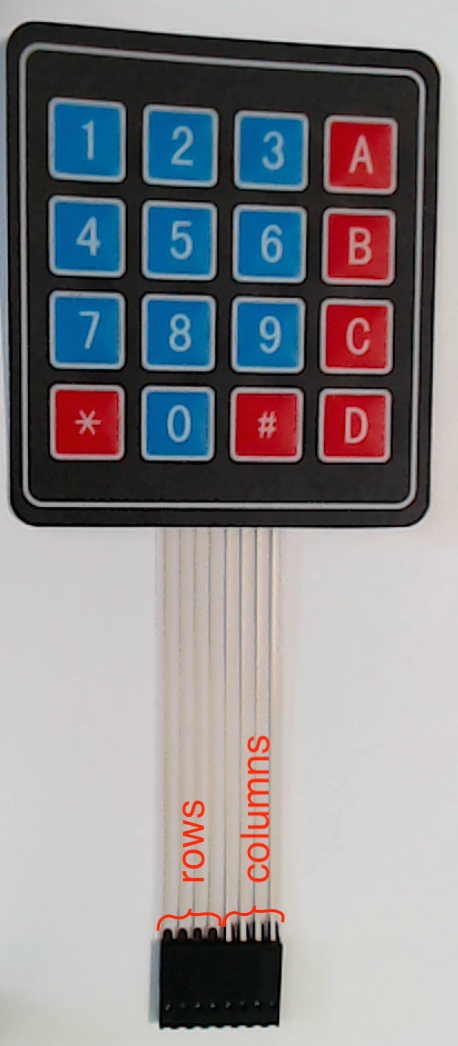
\includegraphics[width=0.25\textwidth]{keypad/keypad-annotated}
%    \caption{The numeric keypad's header has four row pins and four column pins. \label{fig:keypad-annotated}}
%\end{wrapfigure}

Observe that the matrix keypad has sixteen buttons has eight pins in its female connector.
As shown in Figure~\ref{fig:keypad-annotated}, when the keypad is face-up and oriented for reading, the four pins on the left are the \textit{row} pins, and the four pins on the right are the \textit{column} pins.
From left-to-right, we will name these pins \texttt{row1}, \texttt{row4}, \texttt{row7}, \texttt{row*}, \texttt{column1}, \texttt{column2}, \texttt{column3}, \texttt{columnA}.
Figure~\ref{fig:keypad-matrix} shows the membrane contacts and which \developmentboard\ pin will be connected to each keypad pin.

%\begin{wrapfigure}{r}{0.3\textwidth}
%    \centering
%    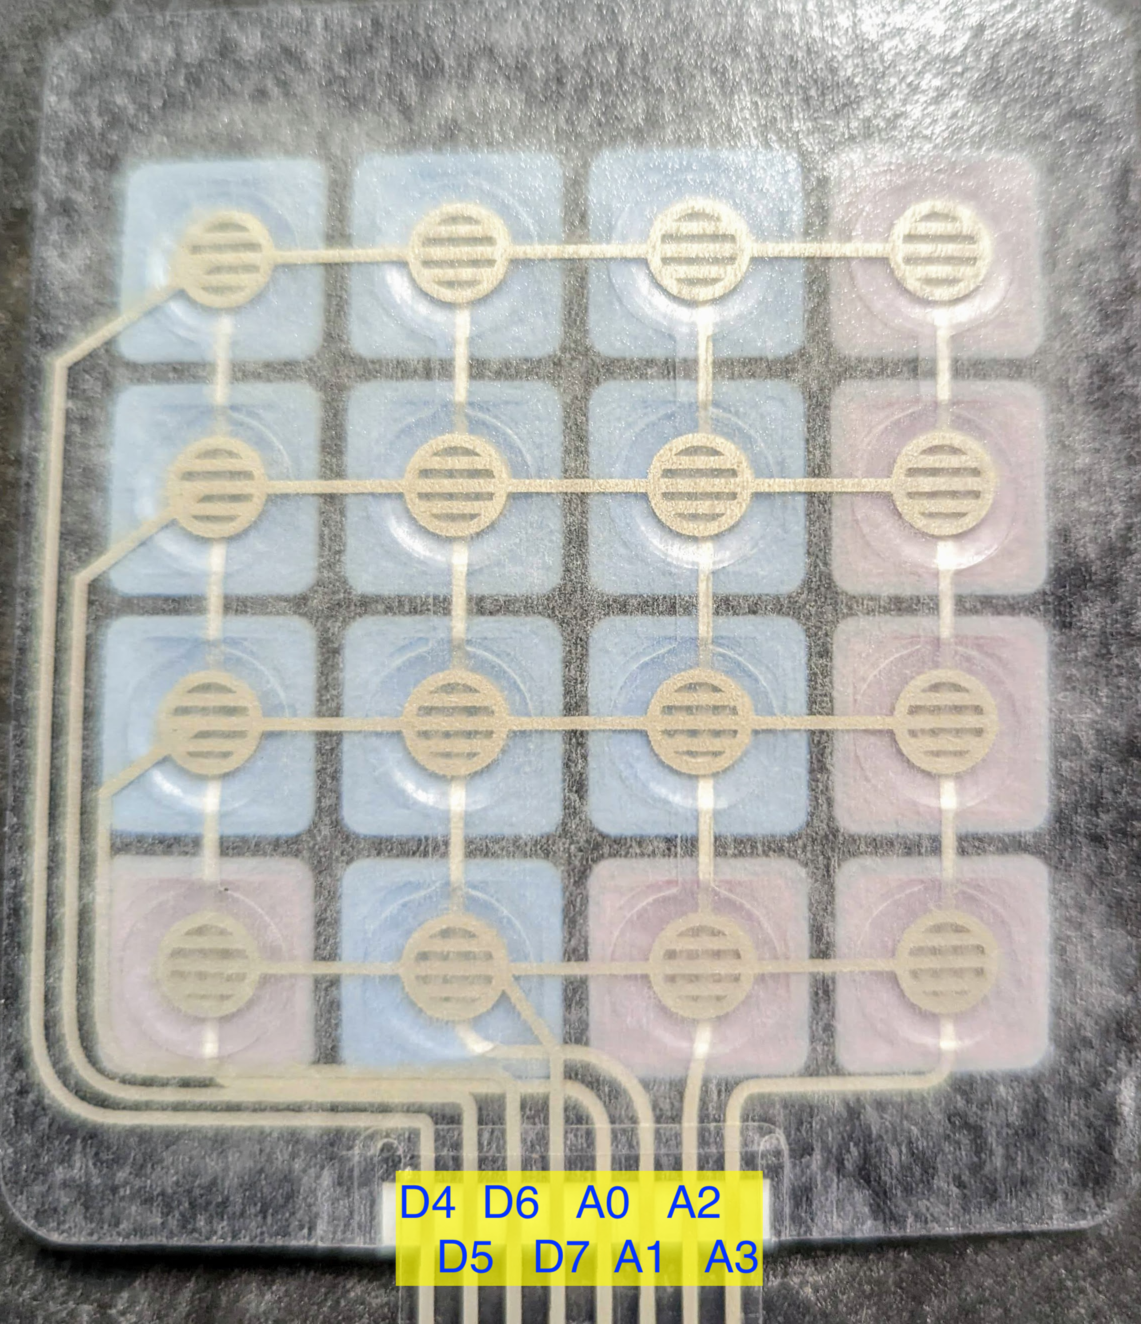
\includegraphics[width=0.25\textwidth]{keypad/keypad-matrix}
%    \caption{The numeric keypad's underlying contact matrix. \label{fig:keypad-matrix}}
%\end{wrapfigure}

\begin{figure}
    \centering
    \subfloat[Front of matrix keypad.] {
        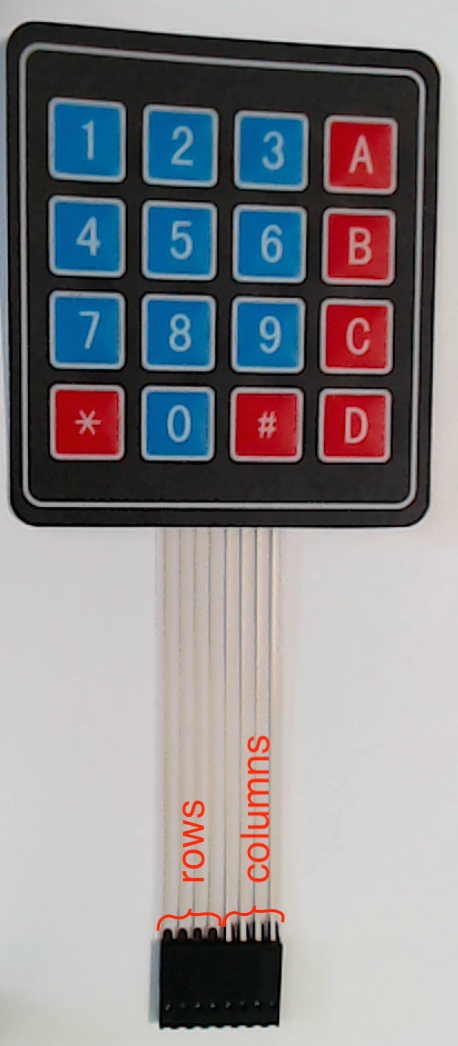
\includegraphics[height=7cm]{keypad/keypad-annotated}
        \label{fig:keypad-annotated}
    }
    \hfil
    \subfloat[Keypad's underlying contact matrix.] {
        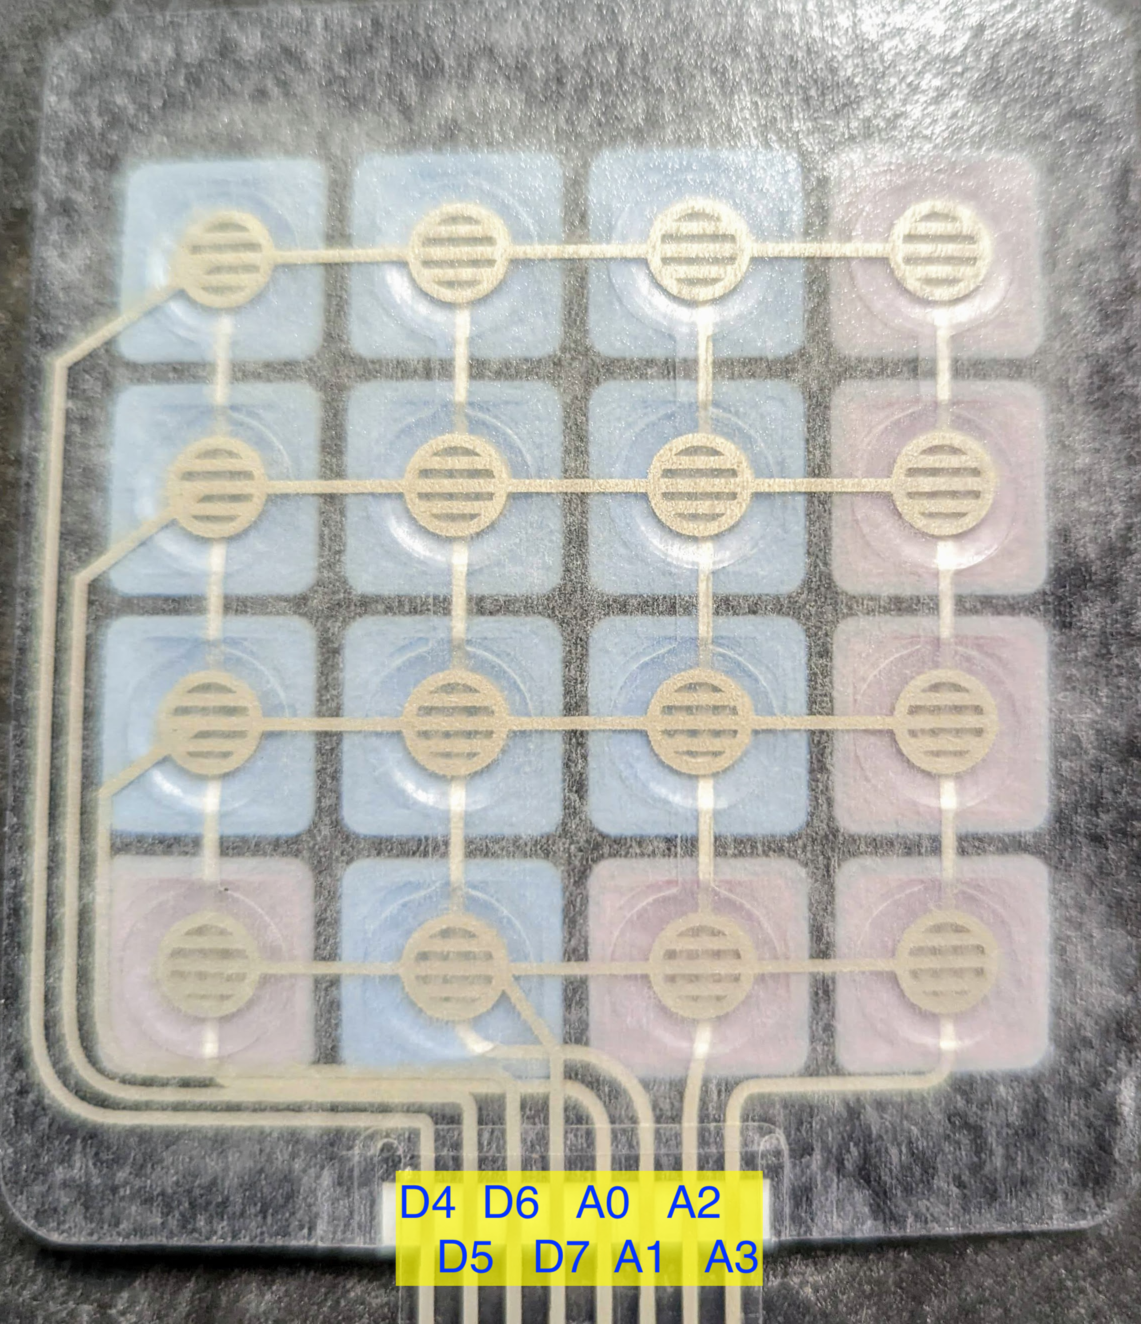
\includegraphics[height=7cm]{keypad/keypad-matrix}
        \label{fig:keypad-matrix}
    }
    \caption{The numeric keypad's header has four row pins and four column pins.}
\end{figure}

Figure~\ref{fig:keypad-diagram} shows a diagram of the wiring for the matrix keypad.

\begin{figure}%[p]
    \centering
    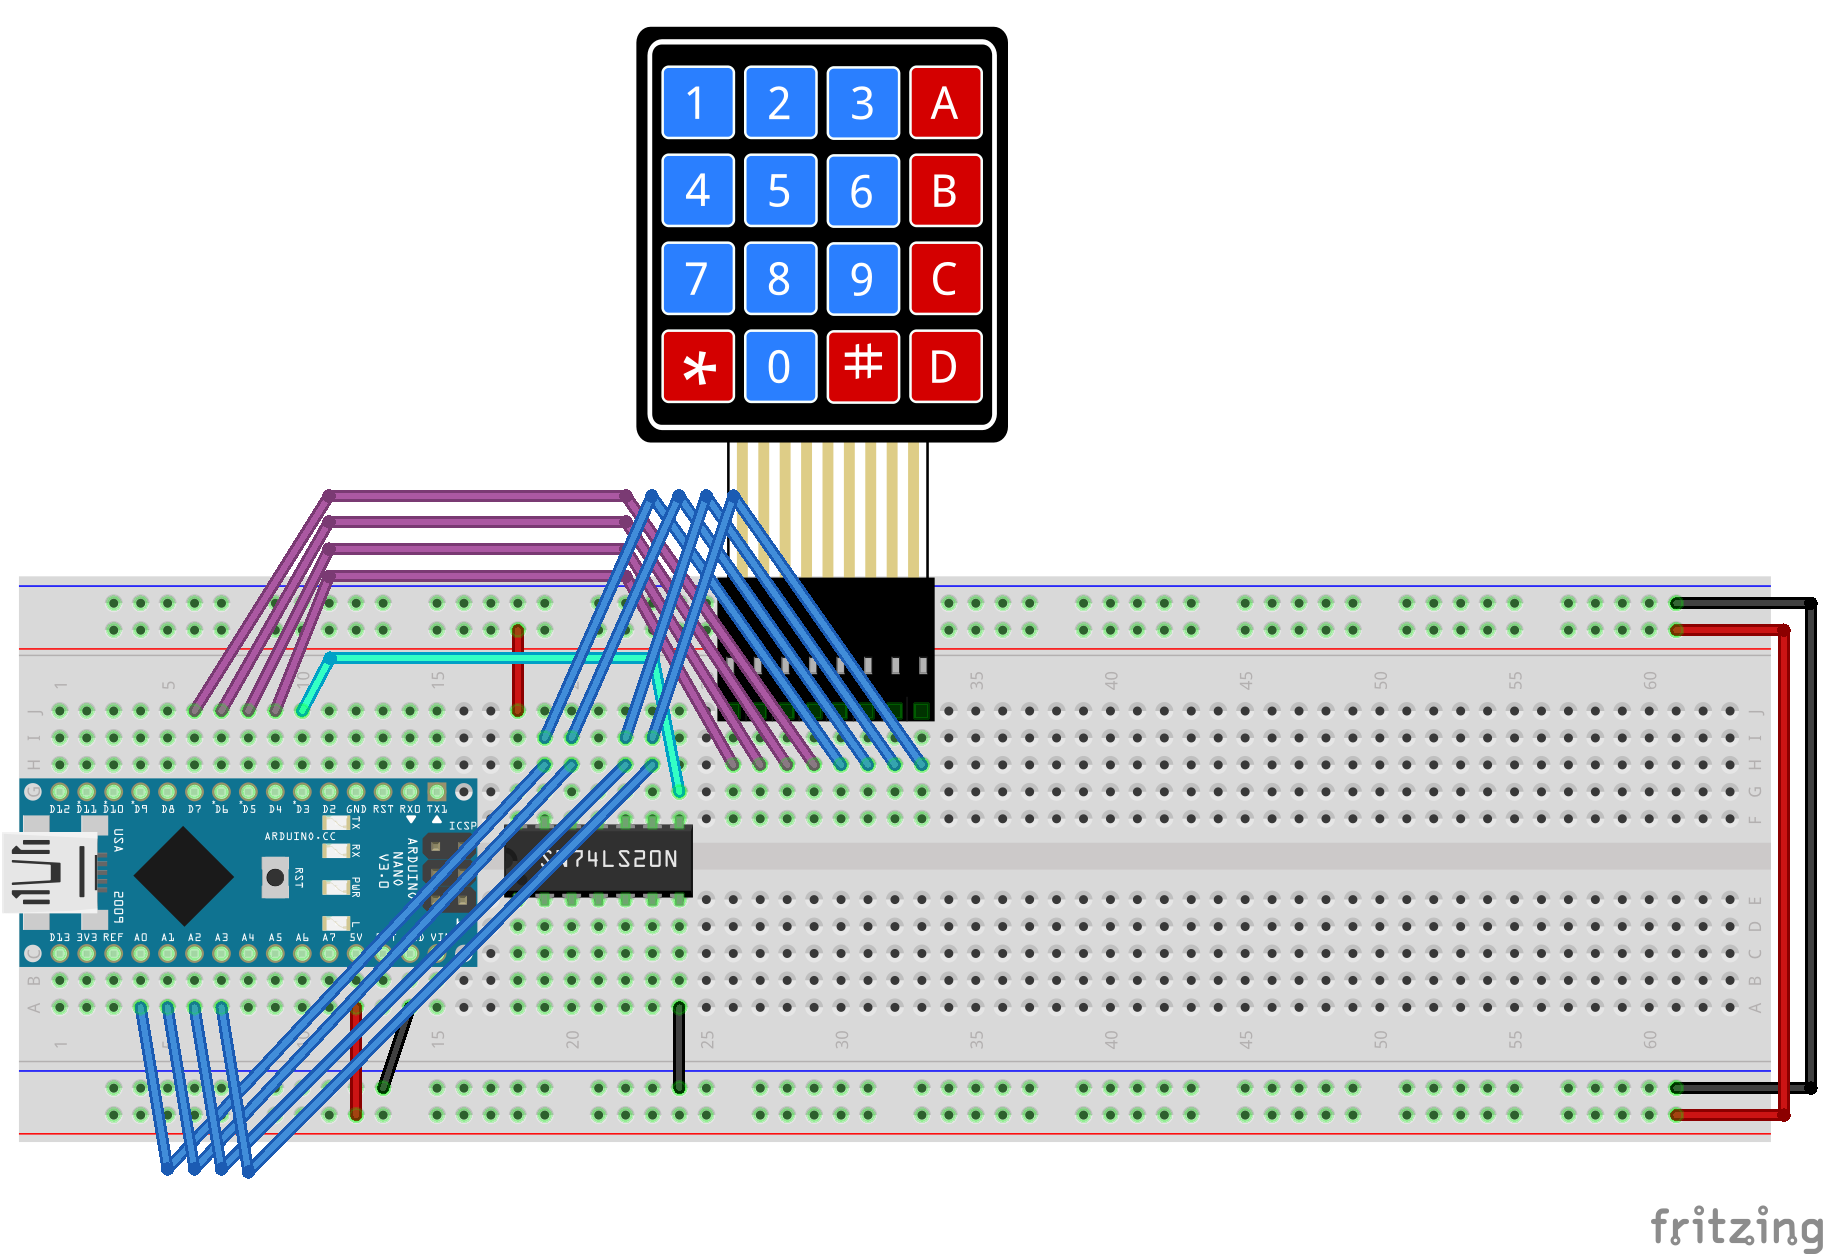
\includegraphics[width=0.9\textwidth]{fritzing_diagrams/keypad}
    \caption{Diagram of wiring associated with matrix keyboard input.
        \textit{Note: connection between the 74LS20's pin 6 and the \developmentboard's
        \texttt{D3} pin was previously installed in Section~\ref{subsec:nand}.}
        \label{fig:keypad-diagram}}
\end{figure}

\disconnect\

\begin{description}
    \checkoffitem{\prepunch{j\controlrow{0}--j\controlrow{7}}
        If your male-male header strip has more than eight pins, then pre-punch additional holes to the right (j\controlrow{8}, j\controlrow{9}, \dots) as needed.}

    \checkoffitem{If your 8-pin male-male header strip is not already inserted into the keypad's female connectors, insert it into the female connectors now.
        If your male-male header strip has more than eight pins, position the excess pins to the right of the column pins.}
    \checkoffitem{Connect your keypad to your breadboard such that \texttt{row1} is in contact point j\controlrow{0}, and \texttt{columnA} is in contact point j\controlrow{7} (and any unused pins on the male-male header are in contact points j\controlrow{8}, j\controlrow{9}, etc.).}
    \item \textbf{NOTE}: if you used 20cm wires to connect your slide-switches and/or pushbuttons to the \developmentboard, then you can use the matrix keypad's ribbon cable to pull these wires away from the circuit, reducing clutter near the controls (Figure~\ref{fig:keypad-pullingwires}).

\begin{figure}
    \centering
    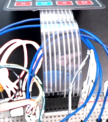
\includegraphics{keypad/keypad-pullingwires}
    \caption{The keypad's ribbon cable can be used to pull long wires out of the way. \label{fig:keypad-pullingwires}}
\end{figure}

    \checkoffitem{Peel off three 4-conductor cables from the \rainbow (Figure~\ref{fig:keypad-cables}).}
    \item While you \textit{can} use individual wires, having these 4-conductor cables will simplify keeping track of the wires.

\begin{figure}
    \centering
    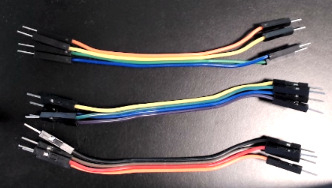
\includegraphics{keypad/keypad-cables}
    \caption{Three 4-conductor cables. \label{fig:keypad-cables}}
\end{figure}

    \checkoffitem{Insert one end of one of the 4-conductor cables in contact points h\controlrow{0}--h\controlrow{3}, in the same breadboard rows as the keypad's row pins.}
    \checkoffitem{Insert the other end of the cable in contact points \mcukeypadrowonepoint--\mcukeypadrowstarpoint.}
    \item You want the \developmentboard's \mcukeypadrowone\ pin to connect to the keypad's \texttt{row1} pin, \mcukeypadrowfour\ to \texttt{row4}, \mcukeypadrowseven\ to \texttt{row7}, and \mcukeypadrowstar\ to \texttt{row*};
        you can use the wires' colors to make sure that you do so.

    \checkoffitem{Insert one end of another 4-conductor cable in contact points h\controlrow{4}--h\controlrow{7}, in the same breadboard rows as the keypad's column pins.}
    \checkoffitem{Insert the other end of the cable in contact points \nandlowerain, \nandlowerbin, \nandlowercin, and \nandlowerdin\ (electrically connected to the 74LS20's \texttt{A1}, \texttt{B1}, \texttt{C1}, and \texttt{D1}: pins 1, 2, 4, and 5).}
    \item \textit{Notice that there are no wires in \nandlowernc} because, as you can see in Figure~\ref{fig:nand-pinout}, the 74LS20's pin 3 is not connected (``NC'') to anything.

    \checkoffitem{Insert one end of the remaining 4-conductor cable in contact points \nandloweraout, \nandlowerbout, \nandlowercout, and \nandlowerdout.}
    \checkoffitem{Insert the other end in contact points \mcukeypadcolonepoint--\mcukeypadcolApoint\ (electrically connected to the \developmentboard's \mcukeypadcolone--\mcukeypadcolA\ pins).}
    \item You want the 74LS20's pin 1 to connect the \developmentboard's \mcukeypadcolone\ pin and the keypad's \texttt{column1} pin, the 74LS20's pin 2 to connect \mcukeypadcoltwo\ and \texttt{column2}, the 74LS20's pin 4 to connect \mcukeypadcolthree\ and \texttt{column3}, and the 74LS20's pin 5 to connect \mcukeypadcolA\ and \texttt{columnA};
        you can use the wires' colors to make sure that you do so.
\end{description}

%\begin{figure}
%    \centering
%    \subfloat[The matrix keypad's connector, with the male-male header strip, just before being inserted into the breadboard.
%        Note the excess header strip's excess pin to the right of the column pins, in contact point j34.]{
%        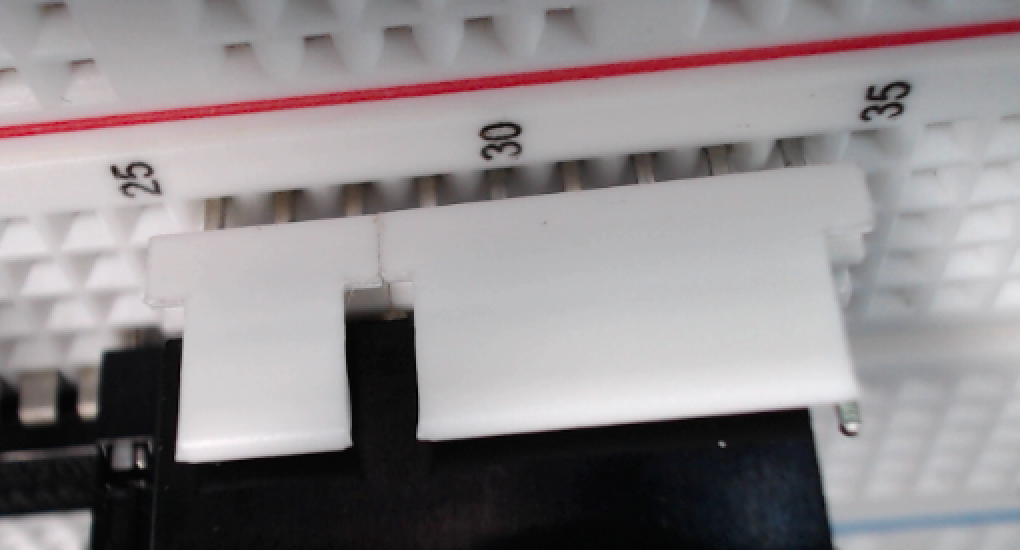
\includegraphics[width=.5\textwidth]{keypad/keypad-header}
%        \label{fig:keypad-header}
%    }
%    \hfil
%    \subfloat[One end of the ``rows'' cable electrically connected to the keypad's row pins.]{
%        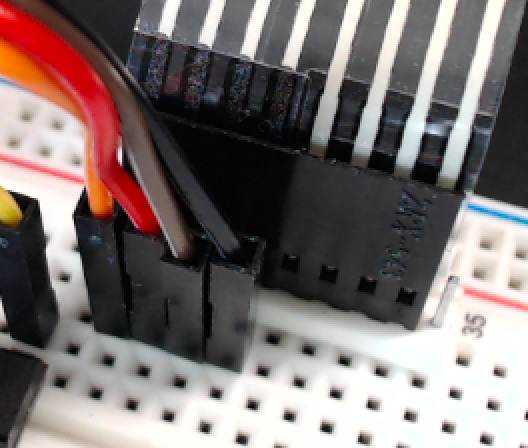
\includegraphics[width=.4\textwidth]{keypad/keypad-row-cable}
%        \label{fig:keypad-row-cable}
%    }
%
%    \subfloat[The other end of the ``rows'' cable electrically connected to the \developmentboard's \texttt{D4}-\texttt{D7} pins.]{
%        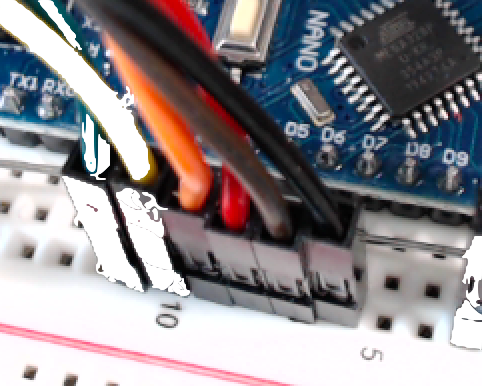
\includegraphics[width=.4\textwidth]{keypad/keypad-row-nano}
%        \label{fig:keypad-row-nano}
%    }
%    \hfil
%    \subfloat[Connection between the keypad's row pins and the \developmentboard's
%        \texttt{D4}-\texttt{D7} pins.]{
%        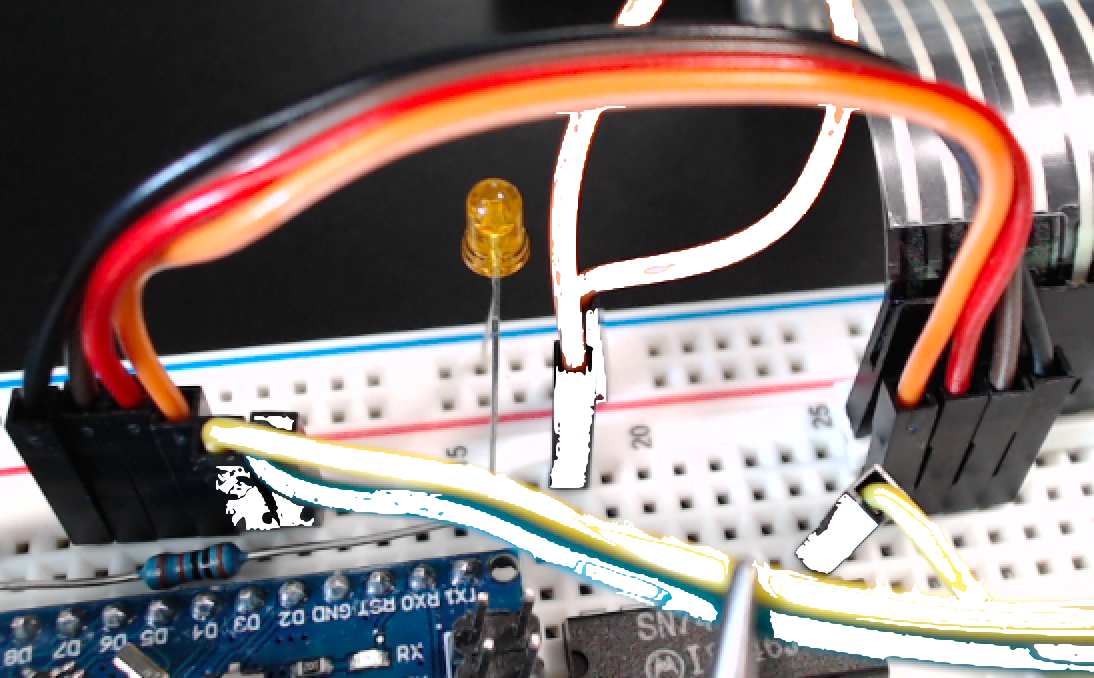
\includegraphics[width=.5\textwidth]{keypad/keypad-row-full}
%        \label{fig:keypad-row-full}
%    }
%
%    \subfloat[Connection between the keypad's column pins and the 74LS20.]{
%        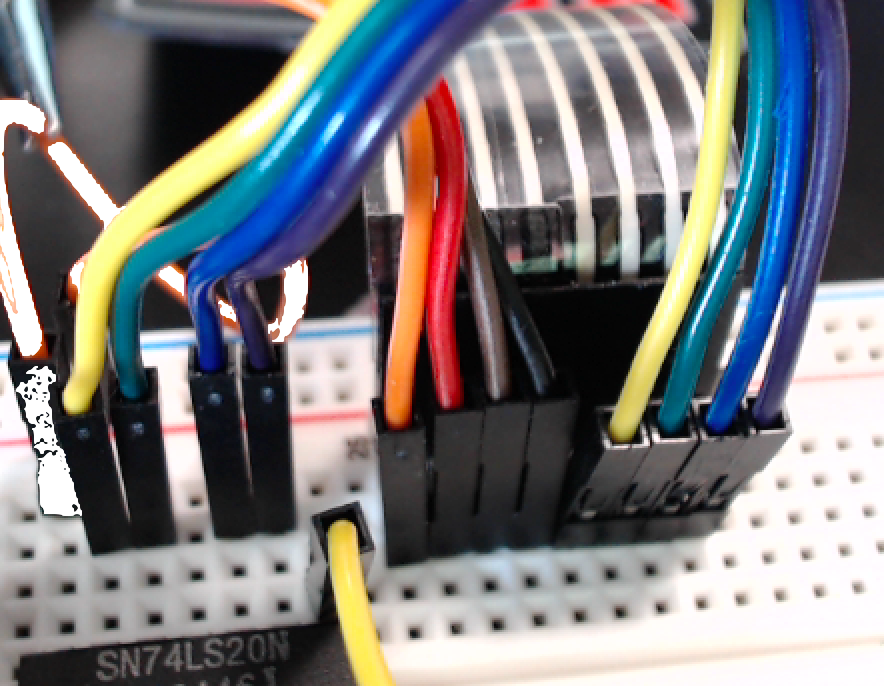
\includegraphics[width=.4\textwidth]{keypad/keypad-col-nand}
%        \label{fig:keypad-col-nand}
%    }
%    \hfil
%    \subfloat[Connection between the the 74LS20 and the \developmentboard's \texttt{A0}-\texttt{A3} pins.]{
%        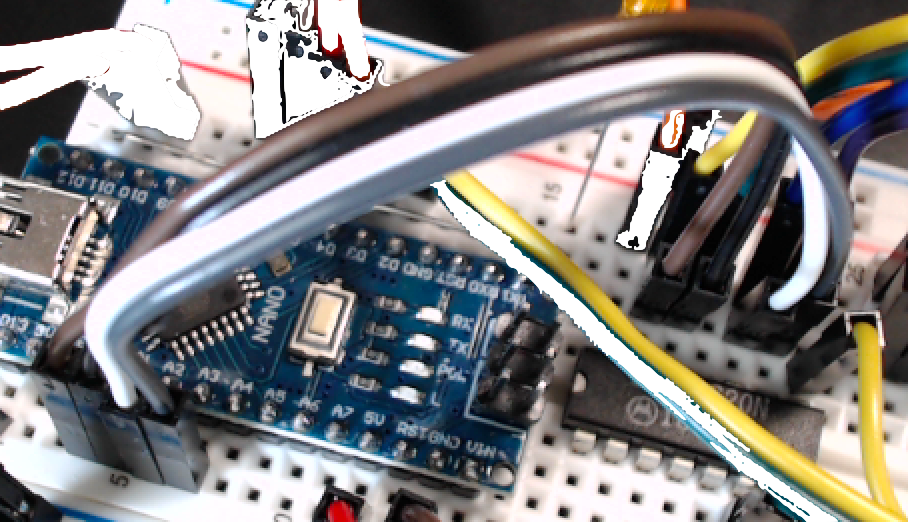
\includegraphics[width=.5\textwidth]{keypad/keypad-col-nano}
%        \label{fig:keypad-col-nano}
%    }
%    \caption{Wiring the Matrix Keypad.}
%\end{figure}

When you have finished setting up the keypad wiring, there should be the electrical paths described in Table~\ref{tab:keypad}.

\begin{table}
    \begin{center}\begin{tabular}{||c|c|c||} \hline\hline
    Keypad pin          & 74LS20            & \developmentboard\ pin \\ \hline
    \texttt{row1}       &                   & \mcukeypadrowone      \\
    \texttt{row4}       &                   & \mcukeypadrowfour     \\
    \texttt{row7}       &                   & \mcukeypadrowseven    \\
    \texttt{row*}       &                   & \mcukeypadrowstar     \\
    \texttt{column1}    & Lower NAND Input  & \mcukeypadcolone      \\
    \texttt{column2}    & Lower NAND Input  & \mcukeypadcoltwo      \\
    \texttt{column3}    & Lower NAND Input  & \mcukeypadcolthree    \\
    \texttt{columnA}    & Lower NAND Input  & \mcukeypadcolA        \\
                        & Lower NAND Output & \mcukeypadnand        \\ \hline
                        & pin 3 (\nandlowernc) & not connected / floating \\ \hline\hline
    \end{tabular}\end{center}
    \caption{Electrical Paths for Matrix Keypad.\label{tab:keypad}}
\end{table}

\checkpoint{inserted and wired the matrix keypad}

\textbf{NOTE:} Do not press more than one key on the matrix keypad at a time.
There are certain combinations of keys that could result in a short-circuit from power to ground, possibly damaging your \developmentboard.
Your \developmentboard\ has some safety measures to prevent damage in that situation, but it would be better for you not to test those safety measures.

Connect your \developmentboard\ to the computer.
In the IDE's Serial Monitor, notice that there is normally no character after \texttt{Keypad:}, that Column~pins is normally 1111, and that Keypad~NAND is normally 0.
Press the 5 key on the matrix keypad.
Notice that the first line of the message from the \developmentboard\ is now
\begin{verbatim}
    Keypad:      5        Column pins:  1011    Keypad NAND: 1
\end{verbatim}
In general, when you press a key on the keypad, the corresponding character will be displayed after \texttt{Keypad:}, and Keypad~NAND will become 1.
When you press 1, 4, 7, or *, Column~pins becomes 0111;
similarly, pressing a key in the 2$^{nd}$ column causes Column~pins to become 1011;
in the 3$^{rd}$ column, 1101;
and in the A$^{th}$ column, 1110.
Be sure to test all 16 keys.
